\section{O Produto}
\label{sec:chap02_product}

Nos últimos anos, o mercado dos sistemas de informação empresariais tem vindo a crescer, sobretudo pela necessidade das empresas aumentarem a sua produtividade e consequentemente, melhorarem a sua competitividade. Embora sistemas \gls{erp} sejam cada vez mais usuais nas empresas, no sentido de gerir as suas operações, estes falham quando aplicados num contexto fabril, ou seja, no \inquotes{chão de fábrica}. Os departamentos produtivos beneficiam de \textit{software} personalizado, que responda às necessidades específicas do foro produtivo/industrial~\parencite{mes_literature_review}. 

Nestas circunstâncias surge o conceito de \gls{mes}, fruto da necessidade das empresas de manufatura progredirem no mercado, num ponto de vista de melhoria da reatividade, da qualidade, dos custo de produção e dos prazos de entrega. Desse modo, as funções de um \gls{mes} estão sobretudo ligadas a atividades de manufatura, que representa uma parte substancial do valor acrescentado em empresas deste setor~\parencite{mes_literature_review}. 

Com o objetivo de apresentar o produto, nesta secção faz-se um enquadramento genérico do conceito \gls{mes} e posteriormente, foca-se o caso específico do {\productname}.

\subsection{\textit{Manufacturing Execution Systems}}

A organização MESA\footnote{\textit{Manufacturing Enterprise Solutions Association}. Disponível em \url{http://www.mesa.org}}, uma comunidade mundial, sem fins lucrativos, que junta empresas de manufatura, de prestação de serviços, analistas, académicos e estudantes, com o propósito de melhorar os resultados do negócio e as operações de produção, através da implementação e implantação de tecnologias de informação e das melhores práticas de gestão, deu o primeiro passo na definição formal de \gls{mes}~\parencite{mes_explained_high_level_vision}:

\begin{quote}
    \inquotes{\textit{Os Manufacturing Execution Systems (MES) fornecem informações que possibilitam a otimização de atividades de produção, desde o lançamento do pedido até aos produtos acabados. Usando dados atualizados e precisos, o MES orienta, inicia, responde e relata as atividades da fábrica à medida que elas ocorrem. A resposta rápida, resultante das mudanças nas condições, associada ao foco na redução de atividades sem valor acrescentado, impulsiona a eficácia das operações e processos fabris. O MES melhora o retorno dos ativos operacionais, bem como o prazo de entrega, gestão de stock, margem bruta e desempenho do fluxo de caixa. O MES fornece informações críticas acerca das atividades de produção em toda a empresa e cadeia logística através de comunicações bidirecionais.}}\footnote{Tradução livre do autor. No original \inquotes{Manufacturing Execution Systems (MES) deliver information that enables the optimization of production activities from order launch to finished goods. Using current and accurate data, MES guides, initiates, responds to, and reports on plant activities as they occur. The resulting rapid response to changing conditions, coupled with a focus on reducing non value-added activities, drives effective plant operations and processes. MES improves the return on operational assets as well as on-time delivery, inventory turns, gross margin, and cash flow performance. MES provides mission-critical information about production activities across the enterprise and supply chain via bi-directional communications.}.}.
\end{quote}

Portanto, o \gls{mes} age como um intermediário entre os diversos processos existentes no \inquotes{chão de fábrica} e os sistemas de \inquotes{alto nível}, existindo comunicação bidirecional entre as camadas, como se demonstra na Figura~\ref{fig:mes_layers}. O \gls{mes} tanto pode fornecer informação acerca dos custos de produção, de indicadores de \textit{performance}, do estado das ordens de fabrico ou rendimento produtivo, como pode também obter dados sobre o planeamento das atividades fabris, parâmetros operacionais, receitas ou instruções de fabrico, por forma a inferir de forma inteligente sobre a fábrica e os seus processos~\parencite{mes_explained_high_level_vision}. Esta bidirecionalidade na comunicação e abrangência no processo produtivo faz com que o \gls{mes} tenha um papel crucial na Indústria $4.0$, já que pode acomodar a integração, descentralização e novas tecnologias, ainda que nem todos os sistemas deste tipo tenham sido desenhados dessa forma~\parencite{cmf_mes_definition}.

\begin{figure}[!ht]
    \centering
    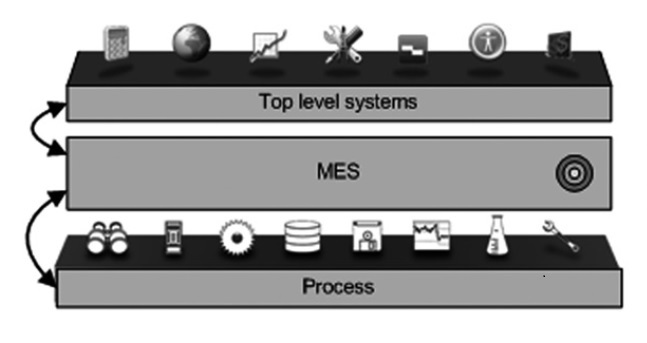
\includegraphics[width=.75\textwidth]{ch02/assets/mes_layers.jpg}
    \caption{Ambiente \glsfirst{mes} e as suas camadas, baseado em~\textcite[p.~526]{mes_literature_review}.}
    \label{fig:mes_layers}
\end{figure}

Com o intuito de dar resposta às necessidades de diversos ambientes produtivos, as funções apresentadas na Figura~\ref{fig:mes_functions} e descriminadas a seguir são essenciais para um \gls{mes}, nomeadamente no suporte, no controlo e na rastreabilidade de cada atividade produtiva~\parencite{mes_literature_review, mes_explained_high_level_vision, introduction_mes}:

\begin{enumerate}
    \item 
    {
        \textit{Operações/Agendamento de detalhes} -- sequenciamento e distribuição temporal das atividades fabris, por forma a otimizar a \textit{performance}, com base nos recursos disponíveis;
    }
    \item
    {
        \textit{Gestão do processo} -- controlo do fluxo de trabalho, baseado nas atividades produtivas reais e planeadas;
    }
    \item
    {
        \textit{Controlo documental} -- gestão e distribuição de informação relativa a produtos, processos, ordens de fabrico, assim como recolher os certificados e condições de trabalho;
    }
    \item
    {
        \textit{Aquisição de dados} -- monitorização, recolha e tratamento de dados sobre os processos, os materiais e operações, por pessoas, máquinas ou controlos;
    }
    \item
    {
        \textit{Gestão laboral} -- supervisão no uso de pessoal de operações num determinado turno, com base nas qualificações, padrões de trabalho e na necessidade de negócio;
    }
    \item
    {
        \textit{Gestão da qualidade} -- registo e análise das características do produto e do processo face aos requisitos ideais;
    }
    \item
    {
        \textit{Expedição de unidades de produção} -- dar a ordem para envio de materiais ou ordens para certos setores da fábrica, com o intuito de iniciar um processo ou sub-processo;
    }
    \item
    {
        \textit{Gestão de manutenção} -- planeamento e execução de tarefas que visam manter o equipamento e outros ativos capazes de executar a sua tarefa, de forma eficaz;
    }
    \item
    {
        \textit{Genealogia e rastreabilidade do produto} -- monitorização do progresso das unidades, amostras ou lotes de saída, para a criação de histórico completo do produto;
    }
    \item
    {
        \textit{Análise de desempenho} -- comparação dos resultados medidos com os objetivos e métricas definidas pela corporação, pelos clientes ou órgãos reguladores;
    }
    \item
    {
        \textit{Estado e alocação de recursos} -- orientação sobre o que as pessoas, máquinas ou ferramentas devem fazer, acompanhando que já fizeram e o que estão a fazer no momento.
    }
\end{enumerate}

\begin{figure}[!ht]
    \centering
    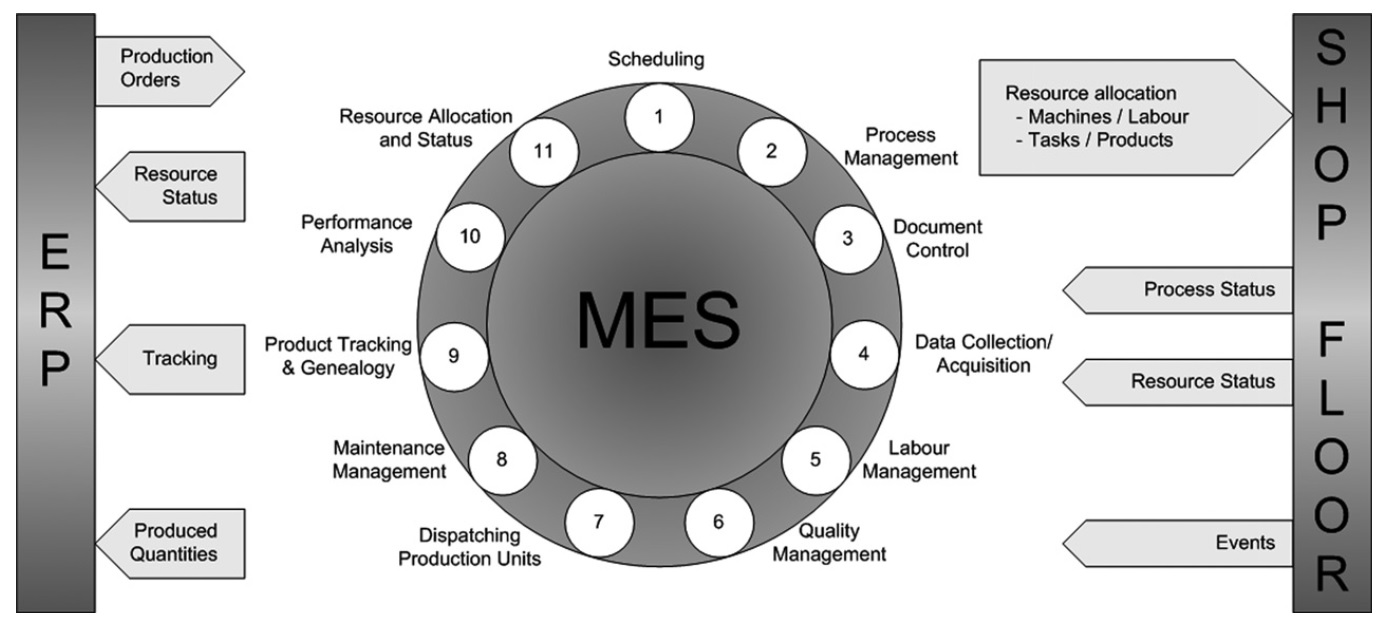
\includegraphics[width=.9\textwidth]{ch02/assets/mes_functions.jpg}
    \caption{Funções do \glsfirst{mes} e o seu enquadramento, extraído de~\textcite{mes_literature_review}}
    \label{fig:mes_functions}
\end{figure}

As funções do \gls{mes} enunciadas servem como base para praticamente qualquer fábrica, fornecendo ferramentas a gestores de fábrica, departamentos de qualidade e manutenção, estando interrelacionadas. Por isso, tratam-se de funções críticas para a maioria dos fabricantes, na medida em que a exigência de processos novos e mais rigorosos no negócio é viável, possibilitando o sucesso no mercado~\parencite{,mes_explained_high_level_vision}. Logo, torna-se evidente que o \gls{mes} traz benefícios para as corporações, alguns alcançáveis num período curto de tempo -- aumento de eficiência e redução de custos; redução no tempo de execução de ordens de fabrico; redução dos custos associados ao trabalho; diminuição ou eliminação de papelada; redução da quantidade de material em processamento; utilização de máquinas mais eficaz --, enquanto que outros, possíveis a longo prazo -- melhoria geral dos processos; maior satisfação do cliente; melhoria na conformidade regulamentar; maior agilidade; melhoria nos prazos de entrega; maior visibilidade da cadeia logística~\parencite{cmf_mes_definition}.

\subsection{{\productname}}

O {\productname} afirma-se como o futuro do \gls{mes}. Trata-se de uma plataforma de \textit{software} inovadora, com um vasto conjunto modular de aplicações e ferramentas, que dotam os utilizadores de indústrias complexas de agilidade, visibilidade e fiabilidade. O produto adapta-se a diversos processos fabris e às suas operações, sendo fácil a sua implantação, independentemente da infraestrutura existente, permitindo o controlo de produção e de custos na empresa e cadeia logística, resultando nas seguintes vantagens~\parencite{cmf_product_overview}:

\begin{enumerate}
    \item 
    {
        Apresenta um \textbf{baixo custo total de posse}\footnote{\textit{Total Cost of Ownership} (TCO). É uma estimativa financeira usada para avaliar os custos diretos e indiretos associados a uma compra.}, visto que a empresa reduz as despesas associadas à implantação, operação e manutenção do sistema;
    }
    \item
    {
        Fornece um largo conjunto de capacidades que dão resposta aos mais variados requisitos, demonstrando a sua \textbf{cobertura funcional};
    }
    \item
    {
        \textbf{Capacita o utilizador na sua função}, sendo este capaz de desenhar e colocar em produtivo o plano da fábrica, rastreando os materiais e os detalhes do processo;
    }
    \item
    {
        É sistema modular, o que o torna \textbf{extensível, flexível e escalável}, dando aos seus utilizadores acesso a inteligência operacional, de forma fácil e rápida; 
    }
    \item
    {
        A arquitetura logicamente descentralizada, ligada à conectividade a diferentes protocolos para equipamentos e dispositivos e ao suporte de produtos preparados para \gls{iot} e \glspl{cps}, tornam o produto \textbf{preparado para a Indústria 4.0}.
    }
\end{enumerate}

Relativamente à arquitetura do produto, demonstrada na Figura~\ref{fig:mes_framework}, a {\companyname} baseou-se nas tecnologias mais
recentes para dotar a sua plataforma da capacidade de adaptação aos diversos ambientes produtivos. Posto isto, a infraestrutura consiste em três camadas, que além de fornecerem particionamento, modularidade e escalabilidade das aplicações, foram projetadas para funcionar em conjunto. Além disso, esta foi desenhada de forma a ser customizável e extensível, dado que cada cliente pode ter os seus próprios requisitos~\parencite{cmf_mes_framework}.

\begin{figure}[!ht]
    \centering
    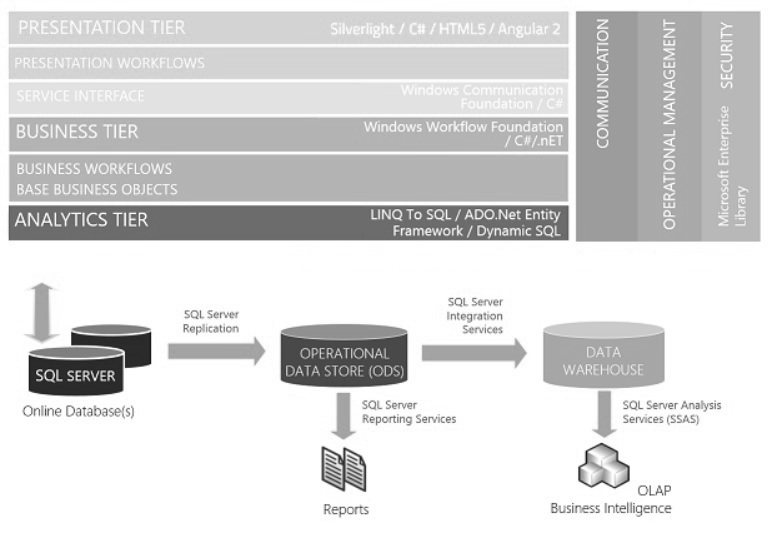
\includegraphics[width=.9\textwidth]{ch02/assets/mes_framework.jpg}
    \caption{Arquitetura do {\productname} e tecnologias usadas, baseado em~\textcite{cmf_mes_framework}}
    \label{fig:mes_framework}
\end{figure}

Quanto às especificidades de cada camada, são descritas de seguida, numa perspetiva de entender a responsabilidade de cada uma delas e o seu contributo para a plataforma~\parencite{cmf_mes_framework}. Já as tecnologias usadas estão especificadas na Figura~\ref{fig:mes_framework}.

\begin{itemize}
    \item 
    {
        \textit{Camada de Apresentação (Presentation Tier)} -- projetada para trazer ao utilizador uma experiência rica e interativa. Dispõe de várias capacidades (\exempligratia{permitir aos utilizadores criar a sua própria interface gráfica ou desenvolver ecrãs para um propósito em particular, numa fábrica ou setor}) e é desenvolvida com suporte multi-plataforma, executando em qualquer sistema operativo \textit{desktop} ou móvel;
    }
    \item
    {
        \textit{Camada de Negócio (Business Tier)} -- implementa e expõe todas as funcionalidades como serviços, estando disponíveis vários protocolos de comunicação. Contém uma sub-camada de orquestração usada para definir os diversos fluxos de negócio, fornecendo a capacidade de coordenação usando os objetos de negócio. Por fim, a sub-camada de objetos de negócio segue um modelo hierárquico, o qual facilita o desenvolvimento de entidades com um comportamento comum;
    }
    \item
    {
        \textit{Camada de Dados (Data Tier)} -- desenhado para suportar as capacidades de armazenamento de dados, possibilitando a integração com fontes de dados externas, geração e modificação de relatórios e mineração de dados.
    }
\end{itemize}

O {\productname} é usado em diversas indústrias, particularmente a indústria de semicondutores~\parencite{cmf_industries_semiconductor}, de equipamentos médicos~\parencite{cmf_industries_medical_devices}, de montagem eletrónica~\parencite{cmf_industries_electronics}, procurando dar resposta aos desafios inerentes a cada uma delas.
